\documentclass{ximera}


\newcommand{\RR}{\mathbb R}
\renewcommand{\d}{\,d}
\newcommand{\dd}[2][]{\frac{d #1}{d #2}}
\renewcommand{\l}{\ell}
\newcommand{\ddx}{\frac{d}{dx}}
\newcommand{\dfn}{\textbf}
\newcommand{\eval}[1]{\bigg[ #1 \bigg]}


\outcome{Define linear approximation as an application of the tangent to a curve.}
\outcome{Find the linear approximation to a function at a point and use it to approximate the function value.}
\outcome{Identify when a linear approximation can be used.}
\outcome{Label a graph with the appropriate quantities used in linear approximation.}
\outcome{Find the error of a linear approximation.}
\outcome{Compute differentials.}
%\outcome{Use the second derivative to discuss whether the linear approximation over or underestimates the actual function value.}
\outcome{Contrast the notation and meaning of $\d y$ versus $\Delta y$.}
%\outcome{Understand that the error shrinks faster than the displacement in the input.}
\outcome{Justify the chain rule via the composition of linear approximations.}


\title[Dig-In:]{Linear approximation}

\begin{document}
\begin{abstract}
We use a method called ``linear approximation'' to estimate the value
of a (complicated) function at a given point.
%  We derive the constant rule, sum rule, power rule, and product rule. 
\end{abstract}
\maketitle

%\section{Linear approximation}

Given a function, a \textit{linear approximation} is a fancy phrase
for something you already know:
\begin{quote}
  \textbf{The line tangent to the graph of a function at a point is very close to the graph of the function near that point.}
\end{quote}
This tangent line is the graph of a linear function, called  the \textbf{linear approximation}.
\begin{example}
Let $f$ be a function that is differentiable on some interval I that contains the point $a$. The graph of a function $f$  and the line tangent to the curve

 $y=f(x)$ at the point where $x=a$ are given in the figure below.
Find the equation of the tangent line.
 \begin{image}
%\begin{marginfigure}
\begin{tikzpicture}
	\begin{axis}[
            xmin=0,xmax=2,ymin=0,ymax=2,
            axis lines=center,
            ticks=none,
            %width=3in,
            %height=2in,
            unit vector ratio*=1 1 1,
            xlabel=$x$, ylabel=$y$,
            every axis y label/.style={at=(current axis.above origin),anchor=south},
            every axis x label/.style={at=(current axis.right of origin),anchor=west},
          ]        
          \addplot [ thick, penColor, smooth, domain=(0:3)] {3*sqrt(x)-2};
          \addplot [thick, penColor2,smooth] {(3/2)*x+3/2-2};
          \node at (axis cs:1.7,1.5) [penColor] {$y=f(x)$};
          \node at (axis cs:1,1.5) [penColor2] {$y=L(x)$}; 
          \node at (axis cs:1.3,1) [penColor2] {$(a,f(a))$}; 
            \addplot[color=penColor3,fill=penColor3,only marks,mark=*] coordinates{(1,1)};  %% closed hole         
        \end{axis}
\end{tikzpicture}
%\caption{A linear approximation of $f(x) = \sin(x)$ at $x=0$.}
%\label{figure:la sin}
%\end{marginfigure}
\end{image}
First, find the expression for $m$, the slope of the tangent line to the curve $y=f(x)$ at the point $(a,f(a))$.
 Select the correct choice.
 \begin{multipleChoice}

 \choice{$m= f(a)$}
  \choice[correct] {$m=f'(a)$}
   \choice{$m= \frac{f(a)-f(0)}{a-0}$}
     \choice{$m= \frac{f(a+h)-f(a)}{h}$}
 \choice{ We don't have enough information to determine the slope.}
  \end{multipleChoice}
Since we know that the point $(a,f(a))$  lies on the tangent line,  we can write an equation of the tangent line. 

\[
y= f'(a)(x-a) +f(a).
\]
Now, we define a function, $L$,  by $L(x)= f'(a)(x-a) +f(a)$. This function is linear and its graph is the line tangent to the curve $y=f(x)$ at the point where $x=a$.
This function deserves a special name.
\end{example}
\begin{definition}\index{linear approximation}
If $f$ is a function differentiable at $x=a$, then a \textbf{linear
  approximation} to the function $f$ at $x=a$ is given by
\[
L(x) = f'(a)(x-a) +f(a).
\]
\end{definition}


Note that the graph of $L$ is just the tangent line to the graph of $f$ at $x=a$.

A linear approximation of $f$ is a ``good'' approximation as long as
$x$ is ``not too far'' from $a$.
%As we see from Figure~\ref{figure:informal-tangent}, 
If one ``zooms in'' on the graph of $f$ sufficiently, then the graphs of $f$ and $L$ 
 are nearly indistinguishable.
 
  As a first example, we
will see how linear approximations allow us to approximate
``difficult'' computations.

\begin{example}
Let $f$ be a function defined by 
\[
f(x) =\sqrt[3]{x}.
\]
Approximate $\sqrt[3]{50}$, using $L$,  a linear approximation to the function $f$ at $a=64$.

\begin{explanation}
To start, write
\[
\ddx f(x) = \ddx x^{1/3} = \frac{1}{3x^{\answer[given]{2/3}}}.
\]
\begin{align*}
L(x) &= \answer[given]{4}+ \frac{1}{3\cdot 64^{2/3}} (x-64)  \\
&=4+ \frac{1}{\answer[given]{48}} (x-64) \\
&= \frac{x}{48} +\frac{8}{3}.
\end{align*}
\begin{image}
%\begin{marginfigure}
\begin{tikzpicture}
	\begin{axis}[
            xmin=0,xmax=100,ymin=0,ymax=5,
            axis lines=center,
             xtick={0, 20, 40, 50, 64, 80, 90, 100},
        xticklabels={0, 20, 40, 50, 64, 80, 90, 100},
            xlabel=$x$, ylabel=$y$,
            every axis y label/.style={at=(current axis.above origin),anchor=south},
            every axis x label/.style={at=(current axis.right of origin),anchor=west},
          ]        
          \addplot [very thick, penColor, samples=150,smooth,domain=(0:100)] {x^(1/3))};
          \addplot [very thick, penColor2, domain=(0:100)] {x/48+8/3};
          \addplot [textColor,dashed] plot coordinates {(64,0) (64,4)};
          \addplot [textColor,dashed] plot coordinates {(0,4) (64,4)};
          \addplot [textColor,dashed] plot coordinates {(50,0) (50,3.68)};
          \node at (axis cs:20,2.3) [penColor] {$f$};
          \node at (axis cs:20,3.3) [penColor2] {$L$};
          \addplot[color=penColor3,fill=penColor3,only marks,mark=*] coordinates{(64,4)};  %% closed hole     
           \addplot[color=penColor,fill=penColor,only marks,mark=*] coordinates{(50,0)};  %% closed hole  
                  
        \end{axis}
\end{tikzpicture}
%\caption{A linear approximation of $f(x) = \sqrt[3]{x}$ at $x=64$.}
%\label{figure:la sqrt3x}
%\end{marginfigure}
\end{image}
Now we evaluate $L(50) \approx 3.71$ and compare it to
$\sqrt[3]{50}\approx 3.68$.  From this we see that the linear
approximation, while perhaps inexact, is computationally \textbf{easier}
than computing the cube root.
\end{explanation}

What would happen if we chose $a=27$ instead?

Then we would use $L_{27}$, the linear approximation to the function $f$ at $a=27$.
In that case, $L_{27}=f(27)+f'(27)(x-27)=3+\frac{1}{27}(x-27)$.
The graph of  $L_{27}$, together with the graphs of $f$ and $L=L_{64}$ is given in the figure below.
\begin{image}
%\begin{marginfigure}
\begin{tikzpicture}
	\begin{axis}[
            xmin=1,xmax=100,ymin=0,ymax=5,
            axis lines=center,
              xtick={0, 27, 40, 50, 64, 80, 90, 100},
        xticklabels={0, 27, 40, 50, 64, 80, 90, 100},
            xlabel=$x$, ylabel=$y$,
            every axis y label/.style={at=(current axis.above origin),anchor=south},
            every axis x label/.style={at=(current axis.right of origin),anchor=west},
          ]        
          \addplot [very thick, penColor, samples=150,smooth,domain=(0:100)] {x^(1/3))};
          \addplot [very thick, penColor2, domain=(0:100)] {x/48+8/3};
            \addplot [very thick, penColor4, domain=(0:100)] {(x-27)/27+3};
              \addplot [textColor,dashed] plot coordinates {(50,0) (50,3.68)};
          \node at (axis cs:6,1.3) [penColor] {$f$};
          \node at (axis cs:20,3.3) [penColor2] {$L_{64}$};
           \node at (axis cs:6,2.5) [penColor4] {$L_{27}$};
          \addplot[color=penColor3,fill=penColor3,only marks,mark=*] coordinates{(64,4)};  %% closed hole         
            \addplot[color=penColor3,fill=penColor4,only marks,mark=*] coordinates{(27,3)};  %% closed hole    
             \addplot[color=penColor3,fill=penColor,only marks,mark=*] coordinates{(50,0)};  %% closed hole     
        \end{axis}
\end{tikzpicture}
%\caption{A linear approximation of $f(x) = \sqrt[3]{x}$ at $x=64$.}
%\label{figure:la sqrt3x}
%\end{marginfigure}
\end{image}
From the picture we can see that 

 $L_{27}(50)>L_{64}(50)>f(50)$.
 
 So, our choice, $a=64$, was better!
\end{example}
With modern calculators and computing software, it may not appear
necessary to use linear approximations. In fact they are quite
useful. In cases requiring an explicit numerical approximation, they
allow us to get a quick rough estimate which can be used as a
``reality check'' on a more complex calculation. In some complex
calculations involving functions, the linear approximation makes an
otherwise intractable calculation possible, without serious loss of
accuracy.

\begin{example}%\label{exam:linear approximation of sine}
Use a linear approximation of $f(x) =\sin(x)$ at $a=0$ to approximate
$\sin(0.3)$.
\begin{explanation}
To start, write
\[
\ddx f(x) = \answer[given]{\cos(x)},
\]
so our linear approximation is
\begin{align*}
L(x) &= 0+\answer[given]{\cos(0)}\cdot(x-0)\\
&= x.
\end{align*}
\begin{image}
%\begin{marginfigure}
\begin{tikzpicture}
	\begin{axis}[
            xmin=-1.6,xmax=1.6,ymin=-1.5,ymax=1.5,
            axis lines=center,
            xtick={-1.57, 0,0.3, 1.57},
            xticklabels={$-\pi/2$, $0$, 0.3, $\pi/2$},
            ytick={-1,1},
            %ticks=none,
            %width=3in,
            %height=2in,
            unit vector ratio*=1 1 1,
            xlabel=$x$, ylabel=$y$,
            every axis y label/.style={at=(current axis.above origin),anchor=south},
            every axis x label/.style={at=(current axis.right of origin),anchor=west},
          ]        
          \addplot [very thick, penColor, samples=100,smooth, domain=(-1.6:1.6)] {sin(deg(x))};
          \addplot [very thick, penColor2, samples=100,smooth] {x};
          \addplot [textColor,dashed] plot coordinates {(0.3,0) (0.3,0.295)};
          \node at (axis cs:1,.7) [penColor] {$f$};
          \node at (axis cs:1,1.18) [penColor2] {$L$};
          \addplot[color=penColor3,fill=penColor3,only marks,mark=*] coordinates{(0,0)};  %% closed hole   
            \addplot[color=penColor3,fill=penColor,only marks,mark=*] coordinates{(0.3,0)};  %% closed hole           
        \end{axis}
\end{tikzpicture}
%\caption{A linear approximation of $f(x) = \sin(x)$ at $x=0$.}
%\label{figure:la sin}
%\end{marginfigure}
\end{image}
Hence, a linear approximation for $\sin(x)$ at $a=0$ is $L(x) = x$,
and so $L(0.3) = 0.3$.  Comparing this to $\sin(.3) \approx 0.295$,
we see that the approximation is quite good. For this reason, it is common
to approximate $\sin(x)$ with its linear approximation $L(x) = x$
when $x$ is near zero.  
%see Figure~\ref{figure:la sin}.
\end{explanation}
\end{example}

\section{Differentials}

The  graph of a function $f$ and the graph of $L$, the linear approximation of $f$ at $a$, are shown in the figure below.
Also, two quantities, $\d x$ and $\d f$, and a point $P$ are marked in the figure. Look carefully at the figure when answering the questions below.


\begin{image}
%\begin{marginfigure}[0in]
\begin{tikzpicture}
	\begin{axis}[
            xmin=1, xmax=2, range=0:6,ymax=6,ymin=0,
            axis lines =left, xlabel=$x$, ylabel=$y$,
            every axis y label/.style={at=(current axis.above origin),anchor=south},
            every axis x label/.style={at=(current axis.right of origin),anchor=west},
            ticks=none,
            axis on top,
          ]         
          \addplot [draw=black,dashed,->,>=stealth'] plot coordinates {(1.4,10/6) (1.7,10/6)};
	  \addplot [draw=black,dashed,->,>=stealth'] plot coordinates {(1.7,10/6) (1.7,10/6 +.3/.36)};
          \addplot [very thick,penColor, smooth,samples=100,domain=(0:1.833)] {-1/(x-2)};
            \addplot [very thick,penColor2, smooth,samples=100,domain=(0:1.833)] {1/0.6+(1/0.36)*(x-1.4)};
  \addplot[color=penColor,fill=penColor,only marks,mark=*] coordinates{(1.7,1/0.3)};  %% closed hole  
   \addplot[color=penColor3,fill=penColor3,only marks,mark=*] coordinates{(1.7,10/6 +.3/.36)};  %% closed hole  
          \addplot[color=penColor3,fill=penColor3,only marks,mark=*] coordinates{(1.4,10/6)};  %% closed hole            
          \node at (axis cs:1.55,1.67) [below] {$\d x$};
          \node at (axis cs:1.7,2.08) [right] {$\d f$};
            \node at (axis cs:1.15,1.85) [below] {$y=f(x)$};
          \node at (axis cs:1.05,0.55) [right] {$y=L(x)$};
           \node at (axis cs:1.24,2.0) [right] {$(a,f(a))$};
            \node at (axis cs:1.478,3.315) [right] {$(x,f(x))$};
              \node at (axis cs:1.68,2.8) [right] {$P$};
        \end{axis}
\end{tikzpicture}
%\caption{While $dy$ and $\d x$ are both variables, $dy$ depends on $\d x$,
  %and approximates how much a function grows after a change of size
  %$\d x$ from a given point.}
%\label{figure:differentials}
%\end{marginfigure}
\end{image}
\begin{question}
  Select all the correct expressions for the quantity $\d x$.
   \begin{hint}
     You can see that $x=a+\d x$.
    \end{hint}
    \begin{selectAll}
      \choice{$\d x=f(x)-f(a)$}
            \choice{$\d x=f(x)-L(x)$}
      \choice[correct]{$\d x=x-a$}
      \choice{$\d x=L(x)-f(a)$}
          \choice{$\d x=L(x)-L(a)$}
    \end{selectAll}
   
  \end{question}
  \begin{question}
  Select all the correct expressions for the quantity $\d f$.
   \begin{hint}
     You can see that $L(x)=f(a)+\d f$.
    \end{hint}
      \begin{hint}
    Recall: $L(a)=f(a)$.
    \end{hint}
    \begin{selectAll}
       \choice{$\d f=f(x)-f(a)$}
            \choice{$\d f=f(x)-L(x)$}
      \choice{$\d f=x-a$}
      \choice[correct]{$\d f=L(x)-f(a)$}
          \choice[correct]{$\d f=L(x)-L(a)$}
         
    \end{selectAll}
   
  \end{question}

 \begin{question}
Based on  the figure and the expression for $L(x)$, select all the correct expressions for $\d f$.
 \begin{hint}
    Recall: $\d f=L(x)-f(a)=f(a)+f'(a)(x-a)-f(a)=f'(a)(x-a)=f'(a)\d x$.
    \end{hint}
      \begin{selectAll}
      \choice[correct]{ $\d f=f'(a)(x-a)$}
      \choice[correct]{ $\d f=f'(a)\d x$}
  \choice{$\d f=f'(x-a)$}
    \choice{$\d f=f'(x)\d x$}
    \choice{$\d f=f'(x)(x-a)$}
      \end{selectAll}
  \end{question}
  
 So, we can write $\d f=f'(a)\d x$ and call it a \textbf{differential} of $f$ at $a$. Notice that we can define a differential at any point $x$ of the domain of $f$, provided that $f'(x)$ exists.
We will  do that in our next definition.
\begin{definition}
Let $f$ be a differentiable function, let $x$ be a point in the domain of $f$, and let  $\d x$ be some quantity, called a \textbf{differential of $x$}.
We define  $\d f$, a differential of $f$,  at a point $x$ by 
\[
\d f=f'(x)\cdot \d x
\] 

 Geometrically, differentials can be interpreted via the diagram below.
\begin{image}
%\begin{marginfigure}[0in]
\begin{tikzpicture}
	\begin{axis}[
            xmin=1, xmax=2, range=0:6,ymax=6,ymin=0,
            axis lines =left, xlabel=$x$, ylabel=$y$,
            every axis y label/.style={at=(current axis.above origin),anchor=south},
            every axis x label/.style={at=(current axis.right of origin),anchor=west},
            ticks=none,
            axis on top,
          ]         
          \addplot [draw=black,dashed,->,>=stealth'] plot coordinates {(1.4,10/6) (1.7,10/6)};
	  \addplot [draw=black,dashed,->,>=stealth'] plot coordinates {(1.7,10/6) (1.7,10/6 +.3/.36)};
          \addplot [very thick,penColor, smooth,samples=100,domain=(0:1.833)] {-1/(x-2)};
            \addplot [very thick,penColor2, smooth,samples=100,domain=(0:1.833)] {1/0.6+(1/0.36)*(x-1.4)};
  \addplot[color=penColor,fill=penColor,only marks,mark=*] coordinates{(1.7,1/0.3)};  %% closed hole  
   \addplot[color=penColor3,fill=penColor3,only marks,mark=*] coordinates{(1.7,10/6 +.3/.36)};  %% closed hole  
          \addplot[color=penColor3,fill=penColor3,only marks,mark=*] coordinates{(1.4,10/6)};  %% closed hole            
          \node at (axis cs:1.55,1.67) [below] {$\d x$};
          \node at (axis cs:1.7,2.08) [right] {$\d f$};
            \node at (axis cs:1.15,1.85) [below] {$f$};
          \node at (axis cs:1.05,0.55) [right] {$L$};
           \node at (axis cs:1.24,2.0) [right] {$(x,f(x))$};
            \node at (axis cs:1.26,3.6) [right] {$(x+\d x,f(x+\d x))$};
          
        \end{axis}
\end{tikzpicture}
%\caption{While $dy$ and $\d x$ are both variables, $dy$ depends on $\d x$,
  %and approximates how much a function grows after a change of size
  %$\d x$ from a given point.}
%\label{figure:differentials}
%\end{marginfigure}
\end{image}

Note, it is now the case (by definition!) that 
\[
 f'(x)=\frac{\d f}{\d x}.
\]
\end{definition}
We should not be surprised, since the slope of the tangent line in the figure is $f'(x)$,  and this slope is also given by $\frac{\d f }{\d x}$.



Essentially, differentials allow us to solve the problems presented in
the previous examples from a slightly different point of view. Recall,
when $h$ is near but not equal zero,
\[
f'(x) \approx \frac{f(x+h)-f(x)}{h}.
\]
Hence, 
\[
f'(x)h \approx f(x+h)-f(x).
\]
We can replace a quantity $h$ with a quantity $\d x$ to write
\begin{align*}
f'(x)\cdot \d x &\approx f(x+\d x)-f(x)\\
\d f &\approx f(x+\d x)-f(x).
\end{align*}
Adding $f(x)$ to both sides we see
\[
f(x) + \d f\approx f(x+\d x)
\]
or, equivalently
\[
f(x+\d x)\approx f(x) + \d f .
\]
There
are contexts where the language of differentials is common. Here is
the basic strategy:
\begin{image}
  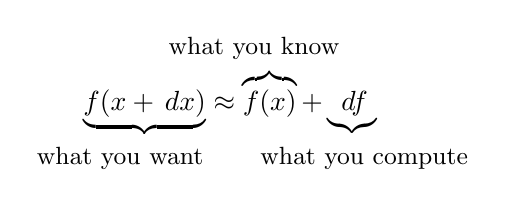
\begin{tikzpicture}
    \node at (0,0) {
      $\underbrace{f(x + \d x)} \approx  \overbrace{f(x)} + \underbrace{\d f}$
    };
    \node at (-1.4,-.7) {\small{what you want}};
    \node at (.3,.7) {\small{what you know}};
    \node at (1.7,-.7) {\small{what you compute}};
  \end{tikzpicture}
\end{image}

We will repeat our previous examples using differentials.

\begin{example}
Use differentials to approximate $\sqrt[3]{50}$.
\begin{explanation}
  Set $f(x) = \sqrt[3]{x}$. We want to know $\sqrt[3]{50}$.  Since
  $4^3 = 64$, we set $x=64$.  Setting $\d x=50-64=-14$, we have
  \begin{align*}
  \sqrt[3]{50} = f(x + \d x) &\approx  f(x) + \d f\\
  &\approx \sqrt[3]{64} + \d f.
  \end{align*}
  Here we see a plot of $y=\sqrt[3]{x}$ with the differentials above
  marked:
  \begin{image}
    \begin{tikzpicture}
      \begin{axis}[
          xmin=40,xmax=70,ymin=3,ymax=4.5,
          axis lines=center,
          xlabel=$x$, ylabel=$y$,
          every axis y label/.style={at=(current axis.above origin),anchor=south},
          every axis x label/.style={at=(current axis.right of origin),anchor=west},
        ]        
        \addplot [very thick, penColor, samples=150,smooth,domain=(0:100)] {x^(1/3))};
        %\addplot [very thick, penColor2, domain=(50:64)] {x/48+8/3};
        %\addplot [textColor,dashed] plot coordinates {(64,0) (64,4)};
        \addplot [draw=black,dashed,->,>=stealth'] plot coordinates {(50,4) (50,3.71)};
        \addplot [draw=black,dashed,->,>=stealth'] plot coordinates {(64,4) (50, 4)};
        \node [above] at (axis cs:57,4) {$\d x$};
        \node [left] at (axis cs:50,3.86) {$\d f$};
        \node [below,penColor3] at (axis cs:64,4) {$(64,4)$};
        \addplot[color=penColor3,fill=penColor3,only marks,mark=*] coordinates{(64,4)};  %% closed hole            
      \end{axis}
    \end{tikzpicture}
    %\caption{A plot of $f(x) = \sqrt[3]{x}$  along with the differentials $\d x$ and $dy$.}
    \label{figure:diff sqrt3x}
  \end{image}
  Now we must compute $\d f$:
  \begin{align*}
    \d f &= f'(x) \cdot \d x\\
    &= \answer[given]{\frac{1}{3x^{2/3}}} \cdot \d x\\
    &= \frac{1}{3\cdot64^{2/3}} \cdot(\answer[given]{-14})\\
    &= \frac{1}{3\cdot64^{2/3}} \cdot(-14)\\
    &= \frac{-7}{24}
  \end{align*}
  Hence $f(50) \approx f(64) + \frac{-7}{24} \approx 3.71$.
\end{explanation}
\end{example}

\begin{example}
Use differentials to approximate $\sin(0.3)$.
\begin{explanation}
Set $y = \sin(x)$. We want to know $\sin(0.3)$. Since $\sin(0) = 0$,
we will set $x = 0$ and $\d x=0.3$. Write with me
\begin{align*}
  \sin(0.3) = \sin(x + \d x) &\approx  \sin(x) + \d y\\
  &\approx 0 + \d y.
  \end{align*}
  Here we see a plot of $y=\sin(x)$ with the differentials above
  marked:
  \begin{image}
%\begin{marginfigure}
\begin{tikzpicture}
	\begin{axis}[
            xmin=-1,xmax=1,ymin=-1,ymax=1,
            axis lines=center,
            xtick={-1.57, 0, 1.57},
            xticklabels={$-\pi/2$, $0$, $\pi/2$},
            ytick={-1,1},
            %ticks=none,
            %width=3in,
            %height=2in,
            unit vector ratio*=1 1 1,
            xlabel=$x$, ylabel=$y$,
            every axis y label/.style={at=(current axis.above origin),anchor=south},
            every axis x label/.style={at=(current axis.right of origin),anchor=west},
          ]        
          \addplot [very thick, penColor, samples=100,smooth, domain=(-1.6:1.6)] {sin(deg(x))};
          %\addplot [penColor2,very thick] plot coordinates {(0,0) (.3,0)};
          %\addplot [penColor2,very thick] plot coordinates {(.3,0) (.3,.3)};
          \addplot [draw=black,dashed,->,>=stealth'] plot coordinates {(0,0) (.3, 0)};
          \addplot [draw=black,dashed,->,>=stealth'] plot coordinates {(.3,0) (.3, .3)};
          \node at (axis cs:.6,.7) [penColor] {$f$};
          \node [below] at (axis cs:.15,.0) {$\d x$};
          \node [right] at (axis cs:.3,.15) {$\d y$};
          \node [above left, color=penColor3] at (axis cs:0,0) {$(0,0)$};
          \addplot[color=penColor3,fill=penColor3,only marks,mark=*] coordinates{(0,0)};  %% closed hole          
        \end{axis}
\end{tikzpicture}
%\caption{A plot of $f(x) = \sin(x)$ along with the differentials $\d x$ and $dy$.}
\label{figure:diff sin}
%\end{marginfigure}
\end{image}
Now we must compute $\d y$:
\begin{align*}
  \d y &= \left(\ddx \sin(x)\right) \cdot \d x\\
  &=\answer[given]{\cos(0)} \cdot \d x\\
  &= 1 \cdot (\answer[given]{0.3})\\
  &= 0.3
\end{align*}
Hence $\sin(0.3) \approx \sin(0) + 0.3 \approx 0.3$.
\end{explanation}
\end{example}

The upshot is that linear approximations and differentials are simply
two slightly different ways of doing the exact same thing.

\section{Error approximation}

Differentials also help us estimate error in real life settings.

\begin{example}
  The cross-section of a $250$ ml glass can be modeled by the function
  $r(x) = \frac{x^4}{3}$:
  \begin{image}
    \begin{tikzpicture}[
        declare function = {f(\x) = (1/3)* pow(\x,4);} ]
      \begin{axis}[
          xmin =-4,xmax=4,ymax=23,ymin=-.2,
          axis lines=center, xlabel=$x$, ylabel=$y$,
          every axis y label/.style={at=(current axis.above origin),anchor=south},
          every axis x label/.style={at=(current axis.right of origin),anchor=west},
          axis on top,
        ]
        \addplot [draw=none,fill=fillp!50!white,domain=-2.65:2.65, smooth] {.8*sqrt(2.65^2-x^2)+16.8} \closedcycle;
        \addplot [draw=none,fill=fillp,domain=-2.65:2.65, smooth] {-.8*sqrt(2.65^2-x^2)+16.8} \closedcycle; 
        \addplot [draw=none,fill=white,domain=-2.7:2.7, smooth] {f(x)} \closedcycle;
        \addplot [ultra thick,penColor, smooth,domain=-2.75:2.75] {f(x)};

        \draw[penColor,very thick] (axis cs:0,16.8) ellipse (265 and 20);
        \draw[penColor,very thick] (axis cs:0,19) ellipse (275 and 20);

        \node[black] at (axis cs:2.5,3) {$y=\frac{x^4}{3}$};       
      \end{axis}
    \end{tikzpicture}
  \end{image}
  At $16.8$ cm from the base of the glass, there is a mark indicating
  when the glass is filled to $250$ ml. If the glass is filled within
  $\pm 2$ millimeters of the mark, what are the bounds on the volume?
  As a gesture of friendship, we will tell you that the volume in
  milliliters, as a function of the height of water in centimeters, $y$,
  is given by
  \[
  V(y) = \frac{2\pi y^{3/2}}{\sqrt{3}}.
  \]
  Note: If you persist in your quest to learn calculus, you will be
  able to derive the formula above like it's no-big-deal.
  \begin{explanation}
    We want to know what a small change in the height, $y$, does to the
    volume $V$.  These small changes can be modeled by the
    differentials $\d V$ and $\d y$. Since
    \[
    \d V = V'(y) \d y
    \]
    and $V'(y) = \answer[given]{\pi \sqrt{3 y}}$ we use the fact that
    $\d y = \pm 0.2$ with $y=\answer[given]{16.8}$ to see
    \[
    \d V = \answer[given]{\pi \sqrt{3 \cdot 16.8}} \cdot 0.2.
    \]
    Hence the volume will vary by at most $\pm\answer[given,tolerance=.01]{4.46062}$
    milliliters.
  \end{explanation}
\end{example}

\section{New and old friends}

You might be wondering, given a plot $y=f(x)$,
\begin{quote}
  What's the difference between $\Delta x$ and $\d x$? What about
  $\Delta y$ and $\d y$?
\end{quote}
Regardless, it is now a pressing question. Here's the deal: 
\[
\frac{\Delta y}{\Delta x}
\]
is the \dfn{average rate of change} of $y=f(x)$ with respect to $x$.
On the other hand:
\[
\frac{\d y}{\d x}
\]
is the \dfn{instantaneous rate of change} of $y=f(x)$ with respect to
$x$. Essentially, $\Delta x$ and $\d x$ are the same type of thing,
they are (usually small) changes in $x$. However, $\Delta y$ and $\d
y$ are very different things.
\begin{itemize}
\item $\Delta y=f(x+\Delta x)-f(x)$; it  is the change in $y=f(x)$ associated to $\Delta x$.
\item $\d y=L(x+\d x)-L(x)$, it is the change in $y=L(x)$ associated to $\Delta x=\d x$.
  \[
  \d y =f'(x)\d x
  \]
  Note: $ L(x+\d x)= f(x)+f'(x)\d x$.
   
  So, the change
  \begin{align*}
    \d y &= L(x+\d x)-L(x)\\
    &= f(x)+f'(x)\d x-L(x)\\
    &= f(x)+f'(x)\d x-f(x)\\
    &=f'(x)\d x
  \end{align*}
\end{itemize}
\begin{question}
  Suppose $f(x) = x^2$. If we are at the point $x=1$ and $\Delta x =\d x
  = 0.1$, what is $\Delta y$? What is $\d y$?
  \begin{hint}
 $ \Delta y=f(1+\Delta x)-f(1)=f(1.1)-f(1)$
    \end{hint}
      \begin{hint}
 $\d y=f'(1)\cdot\d x=f'(1)\cdot0.1$
    \end{hint}
  \begin{prompt}
    \[
    \Delta y = \answer{0.21}\qquad \d y = \answer{0.2}
    \]
  \end{prompt}
\end{question}
Differentials can be confusing at first. However, when you master
them, you will have a powerful tool at your disposal.

\end{document}
